\documentclass[12pt, openany]{book}

\usepackage{graphicx}
\usepackage{caption}
\usepackage{amsmath}
\usepackage{amsfonts}
\usepackage{amssymb}
\usepackage{xcolor}
\usepackage{hyperref}
\usepackage{wrapfig}
\usepackage{cancel}
\usepackage{fancyhdr}
\usepackage{siunitx}
\usepackage{float} 
\usepackage{subcaption}
\usepackage{titlesec}
\titleformat{\chapter}[display]
  {\normalfont\huge\bfseries}
  {\chaptername\ \thechapter}{20pt}{\Huge}
\titlespacing*{\chapter}{0pt}{-10pt}{20pt}
\usepackage[margin=1in]{geometry}

\setlength{\oddsidemargin}{0.025in}
\setlength{\evensidemargin}{0.025in}
\setlength{\textwidth}{6.75in}
\setlength{\topmargin}{0.0in}
\setlength{\textheight}{8.5in}
\setlength{\headheight}{0.25in}
\setlength{\headsep}{0.25in}
\setlength{\topskip}{0.0in}
\setcounter{tocdepth}{3}

\pagestyle{fancy}
\fancyhf{}
\fancyhead[R]{\thepage}  

\title{Albatros Pipeline \\(tentative)}

\author{Thomas Jamieson Bolder}

\begin{document}

\maketitle

\tableofcontents

\chapter{Introduction}


This paper aims to be a resource of informal, high-level documentation on the data analysis pipeline of the ALBATROS low-frequency radio interferometry project. 
It should facilitate outside understanding of the project, whilst providing a solid framework for internal structuring.
This paper is written by a third-year undergraduate in Mathematics and Physics, meaning the level of technical sophistication is reasonably surface-level. 
The author, although having contributed to the project, in no way claims full responsibility for the work outlined here. 

Figure~\ref{fig:project_flow} outlines the general data flow of the overall pipeline.



\begin{figure}[H]
    \centering
    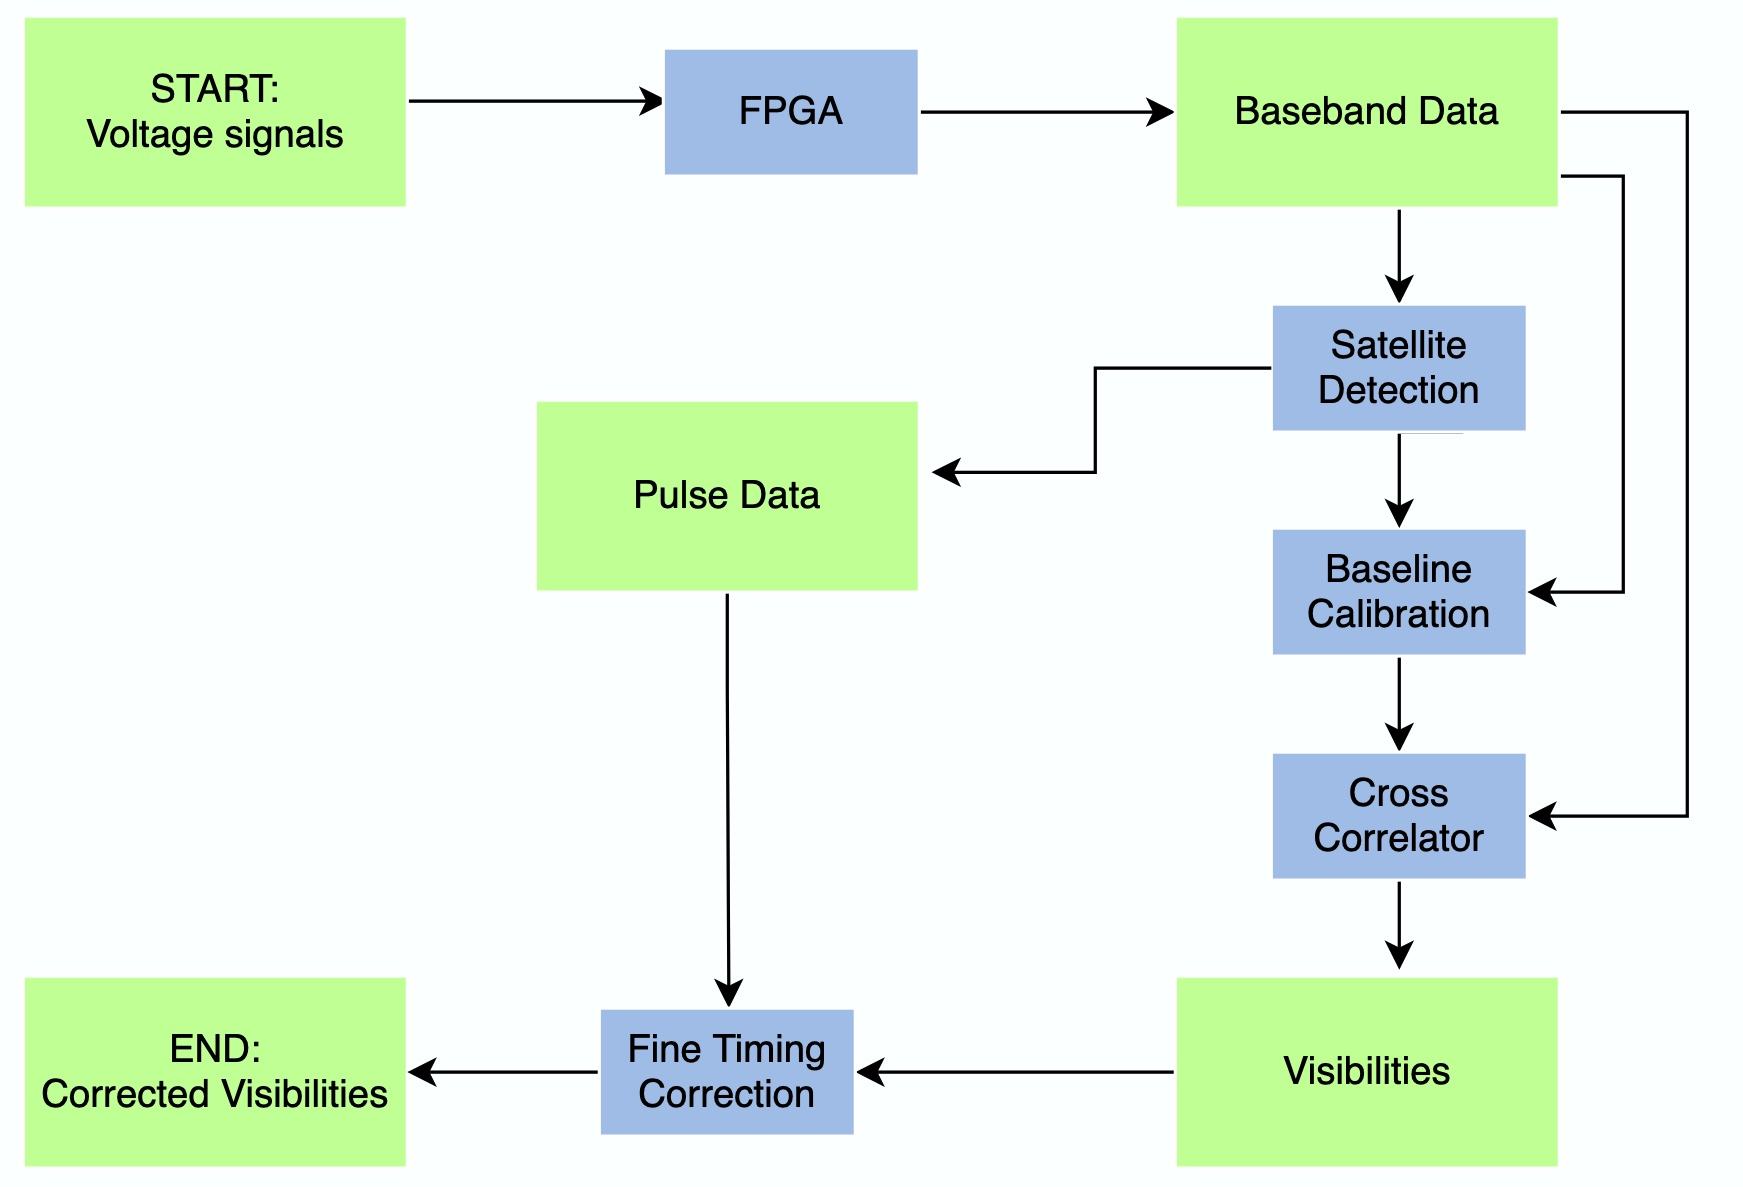
\includegraphics[width=\linewidth]{Figures/project_flow.jpeg}
    \caption{Overall pipeline data flow. Data is in green, whereas processes are in blue.}
    \label{fig:project_flow}
\end{figure}

%add colour and info also. 



\chapter{The Antenna}
\label{chap:antenna}

Here are some things to discuss in this chapter. It's more of a firmware thing (which I am far from being an expert in), useful for some context into how we get our voltages initially.
\begin{itemize}
    \item some details on how the antenna works
    \item polarizations and conventions
    \item the form of data it records
    \item clocks: the RPI clock and the nanosecond iterator. find some name for these guys.
\end{itemize}
Perhaps also discuss the antenna array we are using, as well as the baselines we consider.


\section{Clocks}


Each antenna has a human-time clock in units of unix time, which can drift significantly over the course of a day.

It also has a clock which makes a measurement every 4ns, which is much more reliable but still subject to some jitter.


\chapter{Channelization}

Disuss how we get from voltage to Baseband data. Spectral window, and explain the choices we make.
\chapter{Baseband File System}
\label{chap: baseband}

This chapter is here to give an overview of (and hopefully in more polished versions) give some technical details
into how we store and manipulate baseband data. Not super straightforward, and took me a while to understand.

\begin{itemize}
\item Baseband files are organized by UTC time. 
First the split is by 5 numbers (e.g. 17219), and then split again into raw files of length of about 45 seconds (in the MARS 1 case). 
They have a length of 10 numbers, corresponding to the UTC time at which the measurement of their data \textit{starts}. 
These raw files then contain the FTed data for all our channels, in complex numbers.

\item also note that there are two ways for us to store data, corresponding to different number of bits: 1 bit complex or 4 bit complex 
(corresponding to 2 bits total, or 8 bits total respectively).

\item Since it's an insane amount of data, it is compressed. The way in which it is compressed is in an 8-digit binary, corresponding to either an integer or a complex number. 
unpacking into float complex 64 takes a bunch of time right (explain better too lazy to clean up right away) ('uint8' vs 'complex64')

\item It may also LOSE DATA, so some spectra are missing. This isn't great, but there are functions to help remedy this. 
Make continuous and such are very valuable. Give brief overview, and perhaps link the function page itself.

\end{itemize}
\chapter{Timing}
\label{chap: timing}

\section{Framing the Objective}


With an understanding of the collection and storage of baseband data, we can move on to the question of timekeeping.
The primary issue we must overcome is the misalignment of the human-time clocks in each antenna. 
As mentioned in Chapter~\ref{chap:antenna}, each antenna has a drift-prone human-time clock.
Every time we fetch baseband data at a certain point in unix time, we encounter some unknown offset between 
when we think it was measured and when the data was actually measured.
This is problematic when computing visibilities, since extracting any useful interferometric information 
requires the two timestreams to be perfectly aligned.
However, each antenna also has an internal nano-second iterator, meaning each spectrum (discrete collection of such nano-second iterations)
is almost perfectly (for the purposes of this section) spaced. 
Thus, if we can find the exact offset in spectra between each antenna at a certain point, we know the exact offset 
for the entire day. 
Figure~\ref{fig:offset_diagram} illustrates this visually.
\begin{figure}[H]
    \centering
    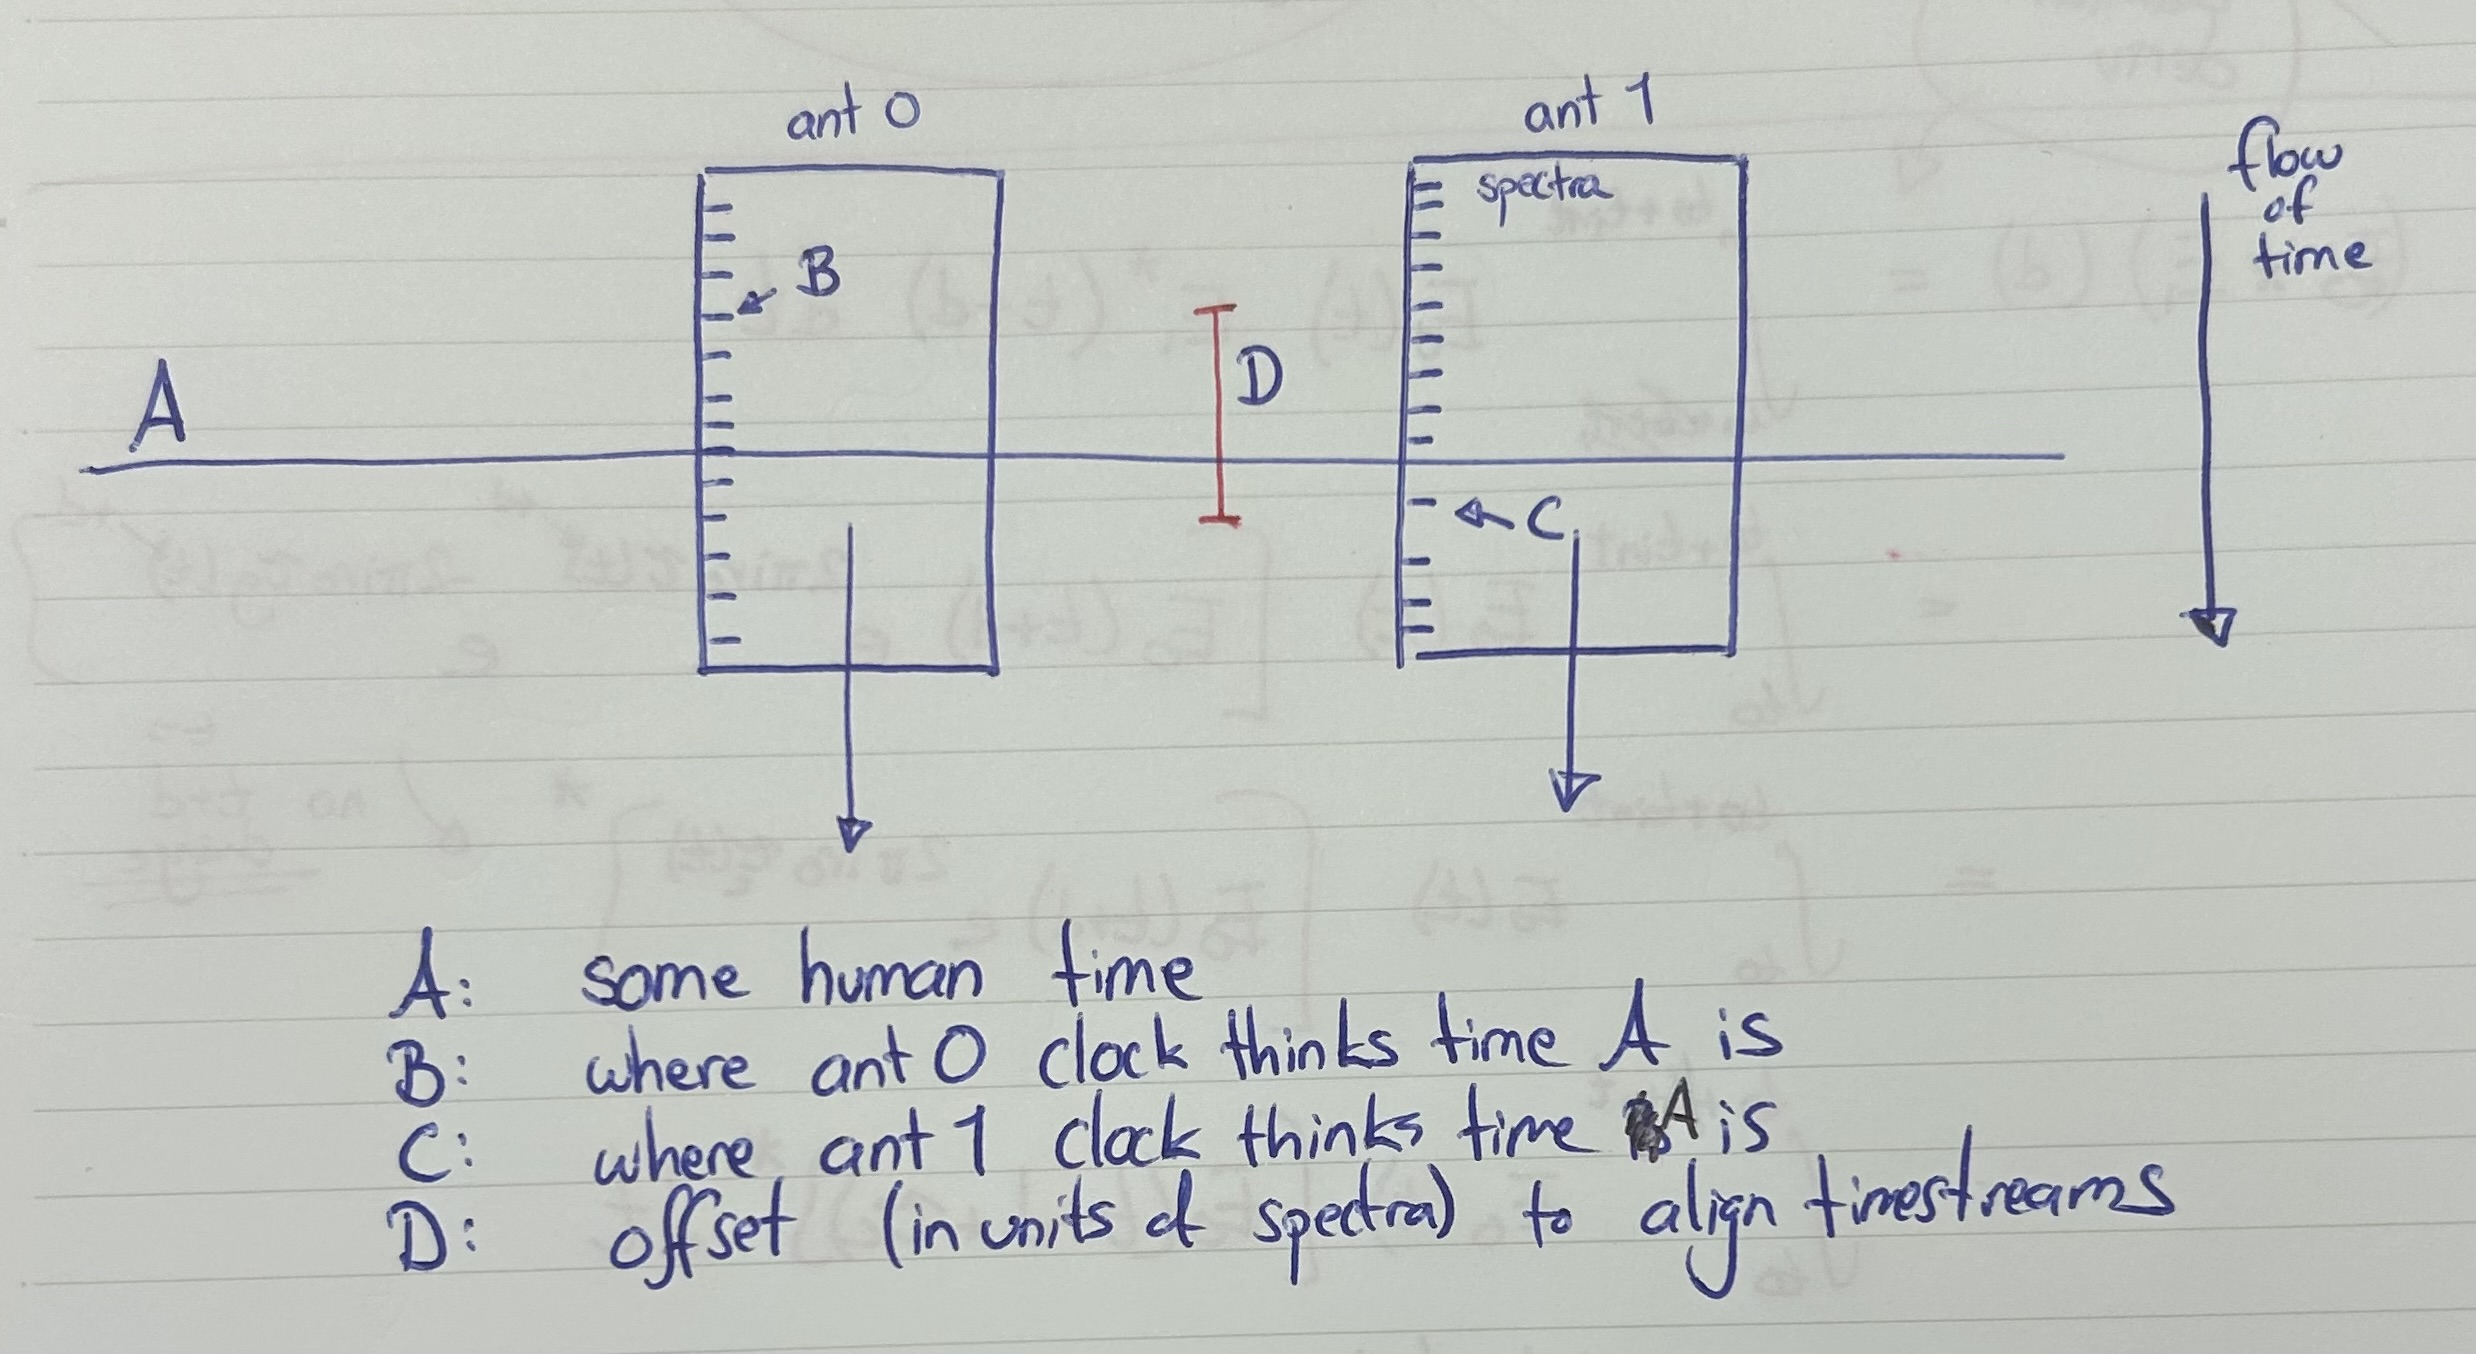
\includegraphics[width=0.7\linewidth]{Figures/offset_diagram.jpg}
    \caption{(Temporary!) Illustration of time offsets in Baseband data timestreams.}
    \label{fig:offset_diagram}
\end{figure}
Note that in this case, the exact observer time loses its significance, since all we really care about is the 
alignment between timestreams. 
We call this game of finding the spectrum index offset between antenna timestreams "spectrum number alignment".


As a side note, since spectra have some finite duration (about 16 $\mu s$ in our case), we cannot align the datastreams
to an infinite level of precision, rather simply to the closest spectrum number integer.  
Despite lacking perfect accuracy, it gives an excellent approximation of the clock offset, leading us into 
more precise corrections later in the analysis (see Chapter~\ref{chap:fine_timing}).


\section{Satellite Passes}

Spectrum number alignment relies on measuring some signal that is visible from both antenna. 
We require a source which: is bright to ensure high SNR, has a known position (for beamforming), 
and has some form of regularity for observation verification.
The best candidates are low orbit satellites, since their signals are strong, their positions are well documented and highly accurate, 
and each satellite passes overhead approximately every 90 minutes. 


Figure~\ref{fig:sat_pulse}   Let us visualize what a satellite pass looks like for two antenna.

\begin{figure}[H]
    \centering
    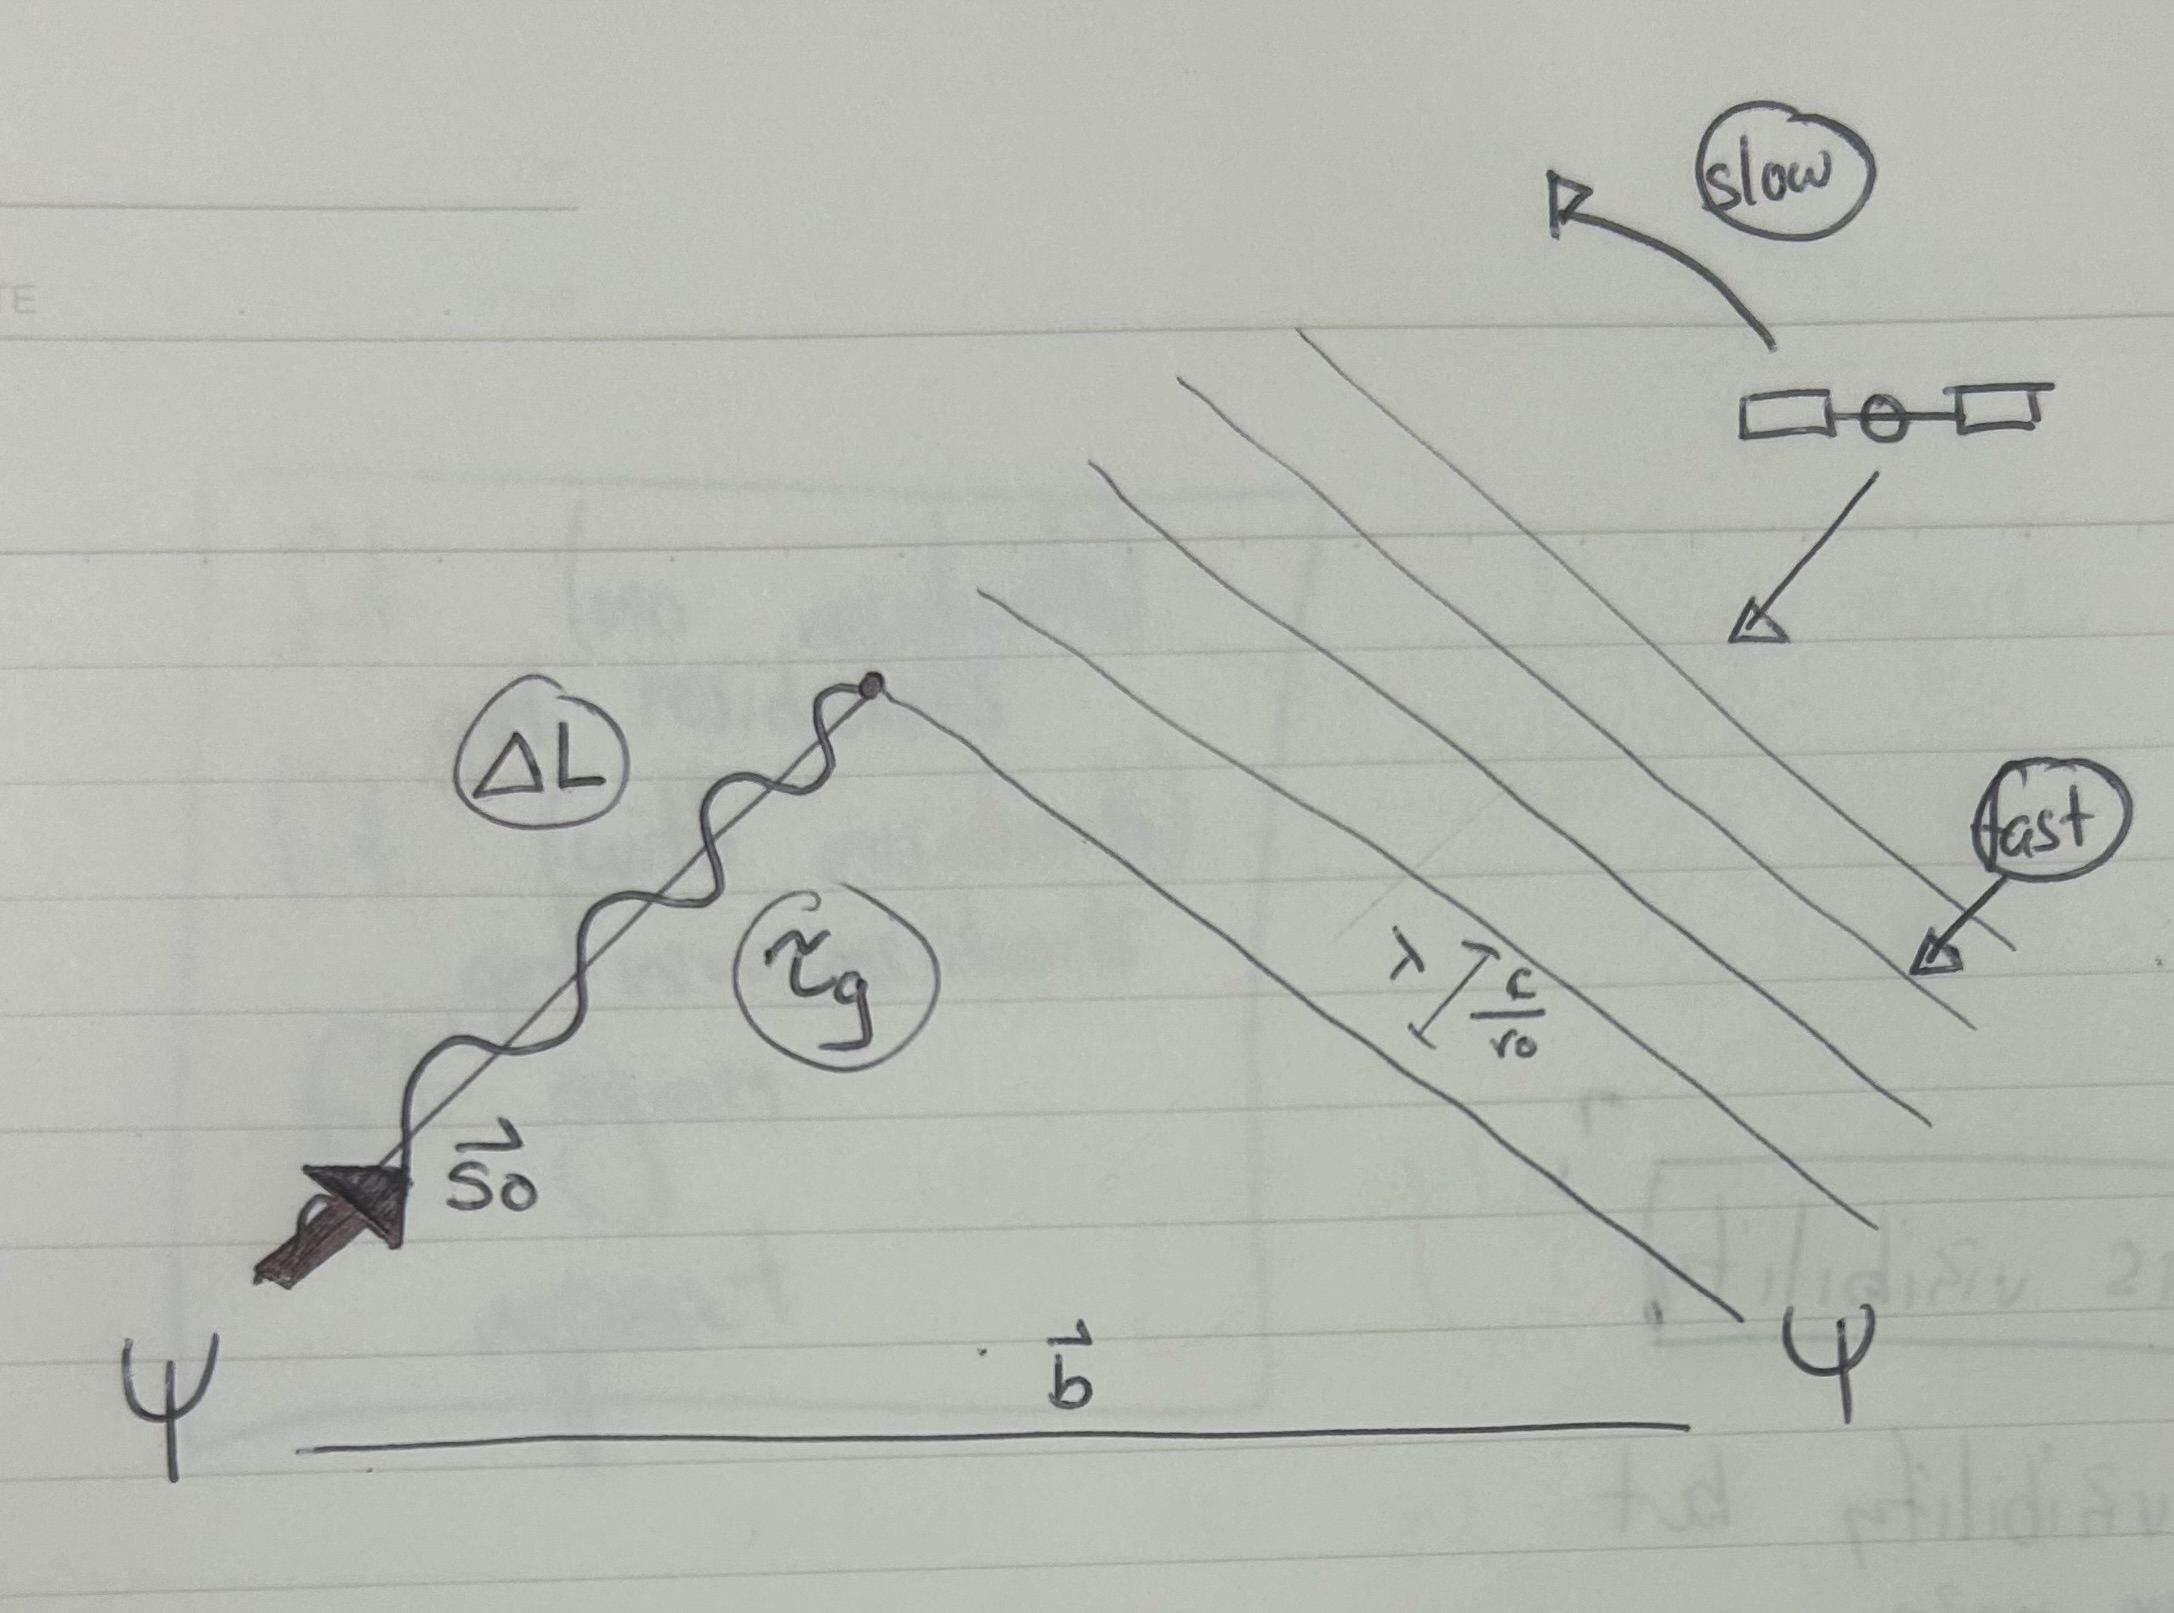
\includegraphics[width=0.7\linewidth]{Figures/sat_det_plot.jpg}
    \caption{(Temporary!) Illustration of a satellite pass}
    \label{fig:sat_pulse}
\end{figure}

Consider a very strong narrowband satellite signal at frequency channel $\nu_0$, in direction $\vec{s_0}$. 
Let us apply the flat sky approximation.
Let us also assume the satellite signal is far brighter than anything else the antenna sees,
such that the sky brightness function $I(\nu, \vec{s})$ is a delta function in the satellite's direction $\vec{s_0}$ 
and at its frequency $\nu_0$. 
We make no assumption on the brightness function in other channels.
Moreover, we also assume the antenna response is uniform.


Let's assume the electric field measured by Antenna 0 is a function of time, $E_0 (t) = a(t) e ^{2 \pi i \nu_0 t}$. 
As we can see in Figure~\ref{fig:sat_pulse}, there is a geometric delay ($\tau_g(t)$)
between the signal arriving at Antenna 0 and Antenna 1, caused by the angle of the satellite in the sky.
Note that $\tau_g(t)$ is a function of time as the satellite's position changes over the duration of its pulse. 
We let the clock offset between the antenna timestreams be $\tau_c(t)$, such that for the satellite signal, 
the total offset between the antenna data streams is $\tau(t) = \tau_c(t) + \tau_g(t)$.
Thus, the signal measured in the Antenna 1 timestream is $E_1 (t) = E_0 e^{2 \pi i \nu_0 \tau(t)}$. 


Our objective here is to find $\tau_c(t)$ given our knowledge of $\tau_g$ (which is easily derived from the satellite's position).
The general idea is removing $\tau_g$ by applying a phase to $E_1$, and then performing a coarse cross-correlation with 
several different spectrum number offsets. 
We are essentially beamforming our antenna towards the expected direction of the satellite, and searching for a signal response. 
The maximal absolute value of the coarse cross-correlation will be attained at the correct offset, as seen below:

\begin{eqnarray}
    (E_0*E_1)(\tau) &=& \int^{t_0 + t_{\text{int}}}_{t_0} E_0(t) E_1^*(t+\tau) dt, \\\nonumber
    &=& \int^{t_0 + t_{\text{int}}}_{t_0} E_0(t) {\left[ E_0(t+\tau) e^{-2\pi i \nu_0 \tau_g(t) + \tau_c(t)} e^{-2\pi i \nu_0 \tau_g(t) } \right]}^* , \\\nonumber
    &=& \int^{t_0 + t_{\text{int}}}_{t_0} E_0(t) {\left[ E_0(t + \tau + \tau_c) \right]}^ *, \\\nonumber
    &=& \int^{t_0 + t_{\text{int}}}_{t_0} E_0(t)  E_0^*(t + \tau + \tau_c)
\end{eqnarray}
Clearly, if $\tau = \tau_c$, we expect the maximal value of the absolute value of the integral, as $E_0$ is correlated with itself. 
It is important to note that we assume both $\tau_c(t)$ and $\tau_g(t)$ remain constant over the course of the cross-correlation.
In general, this holds as the accumulation length $t_{\text{acc}}$ is much smaller than the period of the phasor $e^{2\pi i \nu_0 \tau_g(t)}$.

This approach is a significant simplification of the method far better explained in a document by Mohan Agrawal, found here XX. 

 
As an aside, it is easy to confuse the application of a geometric delay (order 100ns) as being insignificant to a single spectrum
offset (order 16 $\mu s$).
So, why would the removal of 100ns affect a measurement made by shifting in units of 16 $\mu s$?
The geometric delay is better thought of as a phase which compensates for this path difference.
We can easily find the signal arrival's time difference between the antenna, which can be turned into the angle difference
$e^{2 i \pi f \tau_g}$ between the two antenna.
This angle compensation is akin to tilting the (so to say) direction of focus of the antenna.

It is also important to consider that this derivation only holds for the narrowband limit, since a real signal
contains many frequencies. 
Offsets are not quite as simply added for such layered signals.



\section{Practical Implementation}

\subsection{Nomenclature}

Before any correlation can be done, we require accurate and reliable satellite position information. 
The first step of detection is knowing what satellites the antenna can see.
If we know that a satellite is in the field of view of the antenna, we say it is \textbf{risen}. 
The duration over which this satellite is risen is referred to as a \textbf{pass}. 
However, not all risen satellites are visible in the satellite data. 
If we can find the satellite in the correlation of the antenna data, we say it is \textbf{detected}, 
and the duration of time it is risen is a \textbf{pulse}, since we observe a peak in the data for these times. 
Our analysis therefore starts with a long list of risen satellites, with their pass times and satellite ID. 
We aim to detect these. 

Next, TLE files allow us to calculate the geometric delay between the antenna using this TLE file data.
Moreover, if there are multiple satellites present in the pass, applying the different expected geometric delays helps 
differentiate between them.

Thus, we can find a period of data where we know a satellite is risen, and know exactly what the geometric delay is at that time.


\subsection{Discrete Computation}

In practice, spectrum number alignment is done by discrete coarse cross correlation.
We take a chunk of $10^6$ spectra, and consider the central XXXXX spectra.
Since we are shifting the data, we need a buffer such that we don't run out of data for the offset timestream.
We shift the two timestreams by up to 100 000 spectra in either direction, each time correlating these XXXX spectra.
Thus, we end up with 200 001 different correlations (where the extra correlation comes from the zero-offset),
each corresponding to a different spectrum number offset.
Below is the discrete version of one single such correlation, for spectrum number offset k.

\begin{eqnarray}
    (E_0*E_1)(k) &=& \sum_{n=-N}^N E_0[k]E_1^*[n+k]
\end{eqnarray}

Here $N$ is the maximum spectrum offset we will go to, so $N=100000$. 
Figure~\ref{fig:sat_cxcorr_example} shows an example of such a coarse cross-correlation.


\begin{figure}[H]
    \centering
    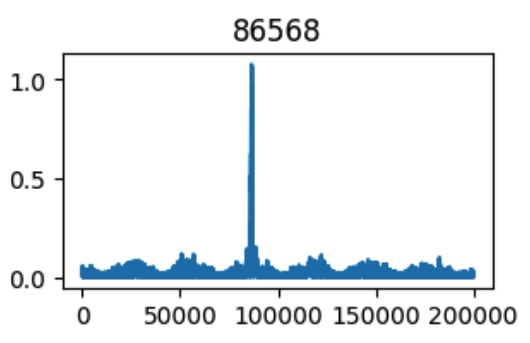
\includegraphics[width=0.5\linewidth]{Figures/american_1.jpeg}
    \caption{A typical cross-correlation for a satellite pass. The x-axis indices are actually -100000 to 100000, 
    matplotlib has just indexed them with natural numbers. The title gives the correlation offset index, 86568, which corresponds to 
    a spectrum number offset of -13432} 
    \label{fig:sat_cxcorr_example}
\end{figure}

There is a clear peak, but as we will later see, this peak may be ambiguous.
Moreover, it is important to realize the spectrum number offset between the antenna, -13432, gives the difference between expected
and measured antenna spectra. 
However, the actual global indices of the antenna are different, and must be adjusted by this value.
For example, let's say the baseband data tells us that at 4pm, Antenna 0 is at spectrum 100000, Antenna 1 is at spectrum 200000, 
and we found an offset of -13432. 
Our convention is that offsets are Ant0 - Ant1, so we know the adjusted global spectrum number offset is 113432.


\section{Analyzing Pulses}

Unfortunately, not all pulses are born equal. 
It turns out that US NORAD satellites have ambiguous peaks, making the spectrum number offset alignment a relatively noisy 
value when considering multiple pulses.
Figure~\ref{fig:american_sats} shows a typical American satellite pulse.


\begin{figure}[H]
    \centering
    \begin{subcaptionbox}{Image 1\label{fig:image1}}[0.3\textwidth]
        {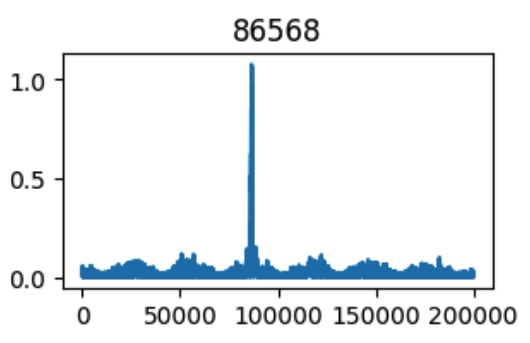
\includegraphics[width=\linewidth]{Figures/american_1.jpeg}}
    \end{subcaptionbox}
    \hfill
    \begin{subcaptionbox}{Image 2\label{fig:image2}}[0.3\textwidth]
        {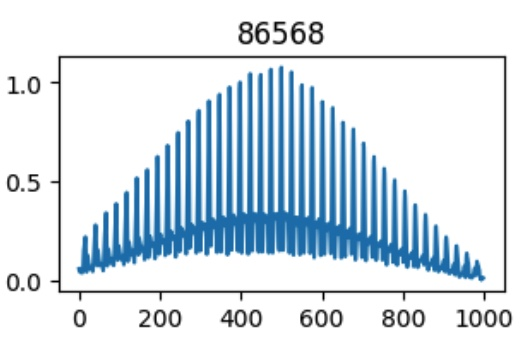
\includegraphics[width=\linewidth]{Figures/american_2.jpeg}}
    \end{subcaptionbox}
    \hfill
    \begin{subcaptionbox}{Image 3\label{fig:image3}}[0.3\textwidth]
        {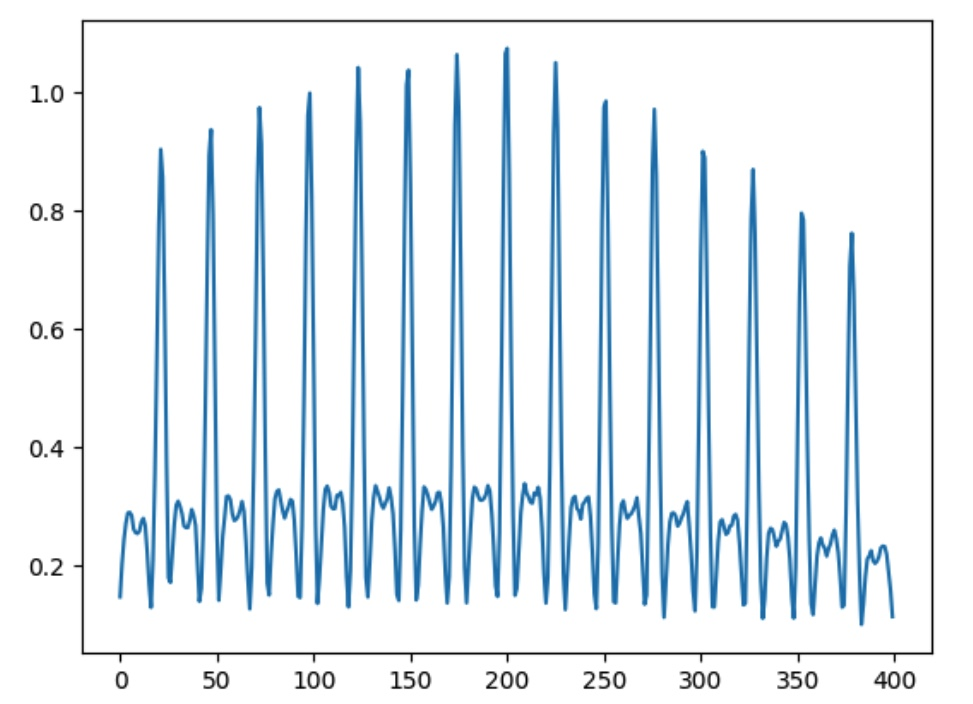
\includegraphics[width=\linewidth]{Figures/american_3.jpeg}}
    \end{subcaptionbox}
    \caption{A usual American satellite pulse. Left is most zoomed out, right is most zoomed in. Can see the periodic peaks.}
    \label{fig:american_sats}
\end{figure}

At high resolution, the peak consists of several smaller, sharp peaks. This means the offset can often get confused.

Fortunately, Russian satellites have a strong and distinct pulse in the coarse cross correlation, as seen in Figure~\ref{fig:russian_sats}.


%\begin{figure}[H]
%    \centering
%   \begin{subcaptionbox}{Image 1\label{fig:image1}}[0.3\textwidth]
%        {\includegraphics[width=\linewidth]{image1.jpg}}
%    \end{subcaptionbox}
%    \hfill
%    \begin{subcaptionbox}{Image 2\label{fig:image2}}[0.3\textwidth]
%        {\includegraphics[width=\linewidth]{image2.jpg}}
%    \end{subcaptionbox}
%    \hfill
%    \begin{subcaptionbox}{Image 3\label{fig:image3}}[0.3\textwidth]
%        {\includegraphics[width=\linewidth]{image3.jpg}}
%    \end{subcaptionbox}
%    \caption{A usual Russian satellite pulse. Left is most zoomed out, right is most zoomed in. Can see the sharp peak.}
%    \label{fig:three_images}
%\end{figure}
 
Clearly, such Russian peaks are far better for spectrum number alignment.
We can differentiate between them using what we call a \textbf{reliability ratio}.
This crude but effective method provides a measure of the sharpness of the peak.
It zooms into the closest 200 spectra from the main peak and finds the position of the five next-tallest peaks.
It then find the mean (normalized) difference between the main peak and the other next-tallest peaks.
If this value is high, then there are likely other similarly sized peaks bunched together, indicating an American-style pulse.
If this value if low, then there is only a single dominant peak, and we can trust the offset value it provides.
The reliability ratio is recorded alongside all other pulse information in the detection process.






\chapter{Baseline Calibration}

\section{Framework}
%I might want to include more detail about how accurate we want it to be. Like including errors or something.

At this point in the pipeline, the positional coordinates of each antenna are only known to approximate values. Since interferometry is heavily reliant on highly accurate baseline vectors, using such rough coordinates would yield unsatisfactory visibilities. Therefore, we must calibrate our antenna baselines as a preliminary step for further data analysis. As we will explore in more detail in the following sections, the calibration process itself is performed by minimizing phase residuals between observed and predicted satellite passes. Let us first visualize what our antenna array might look like with an example shown in Figure~\ref{fig:ant_cluster}.

\begin{figure}[H]
  \centering
  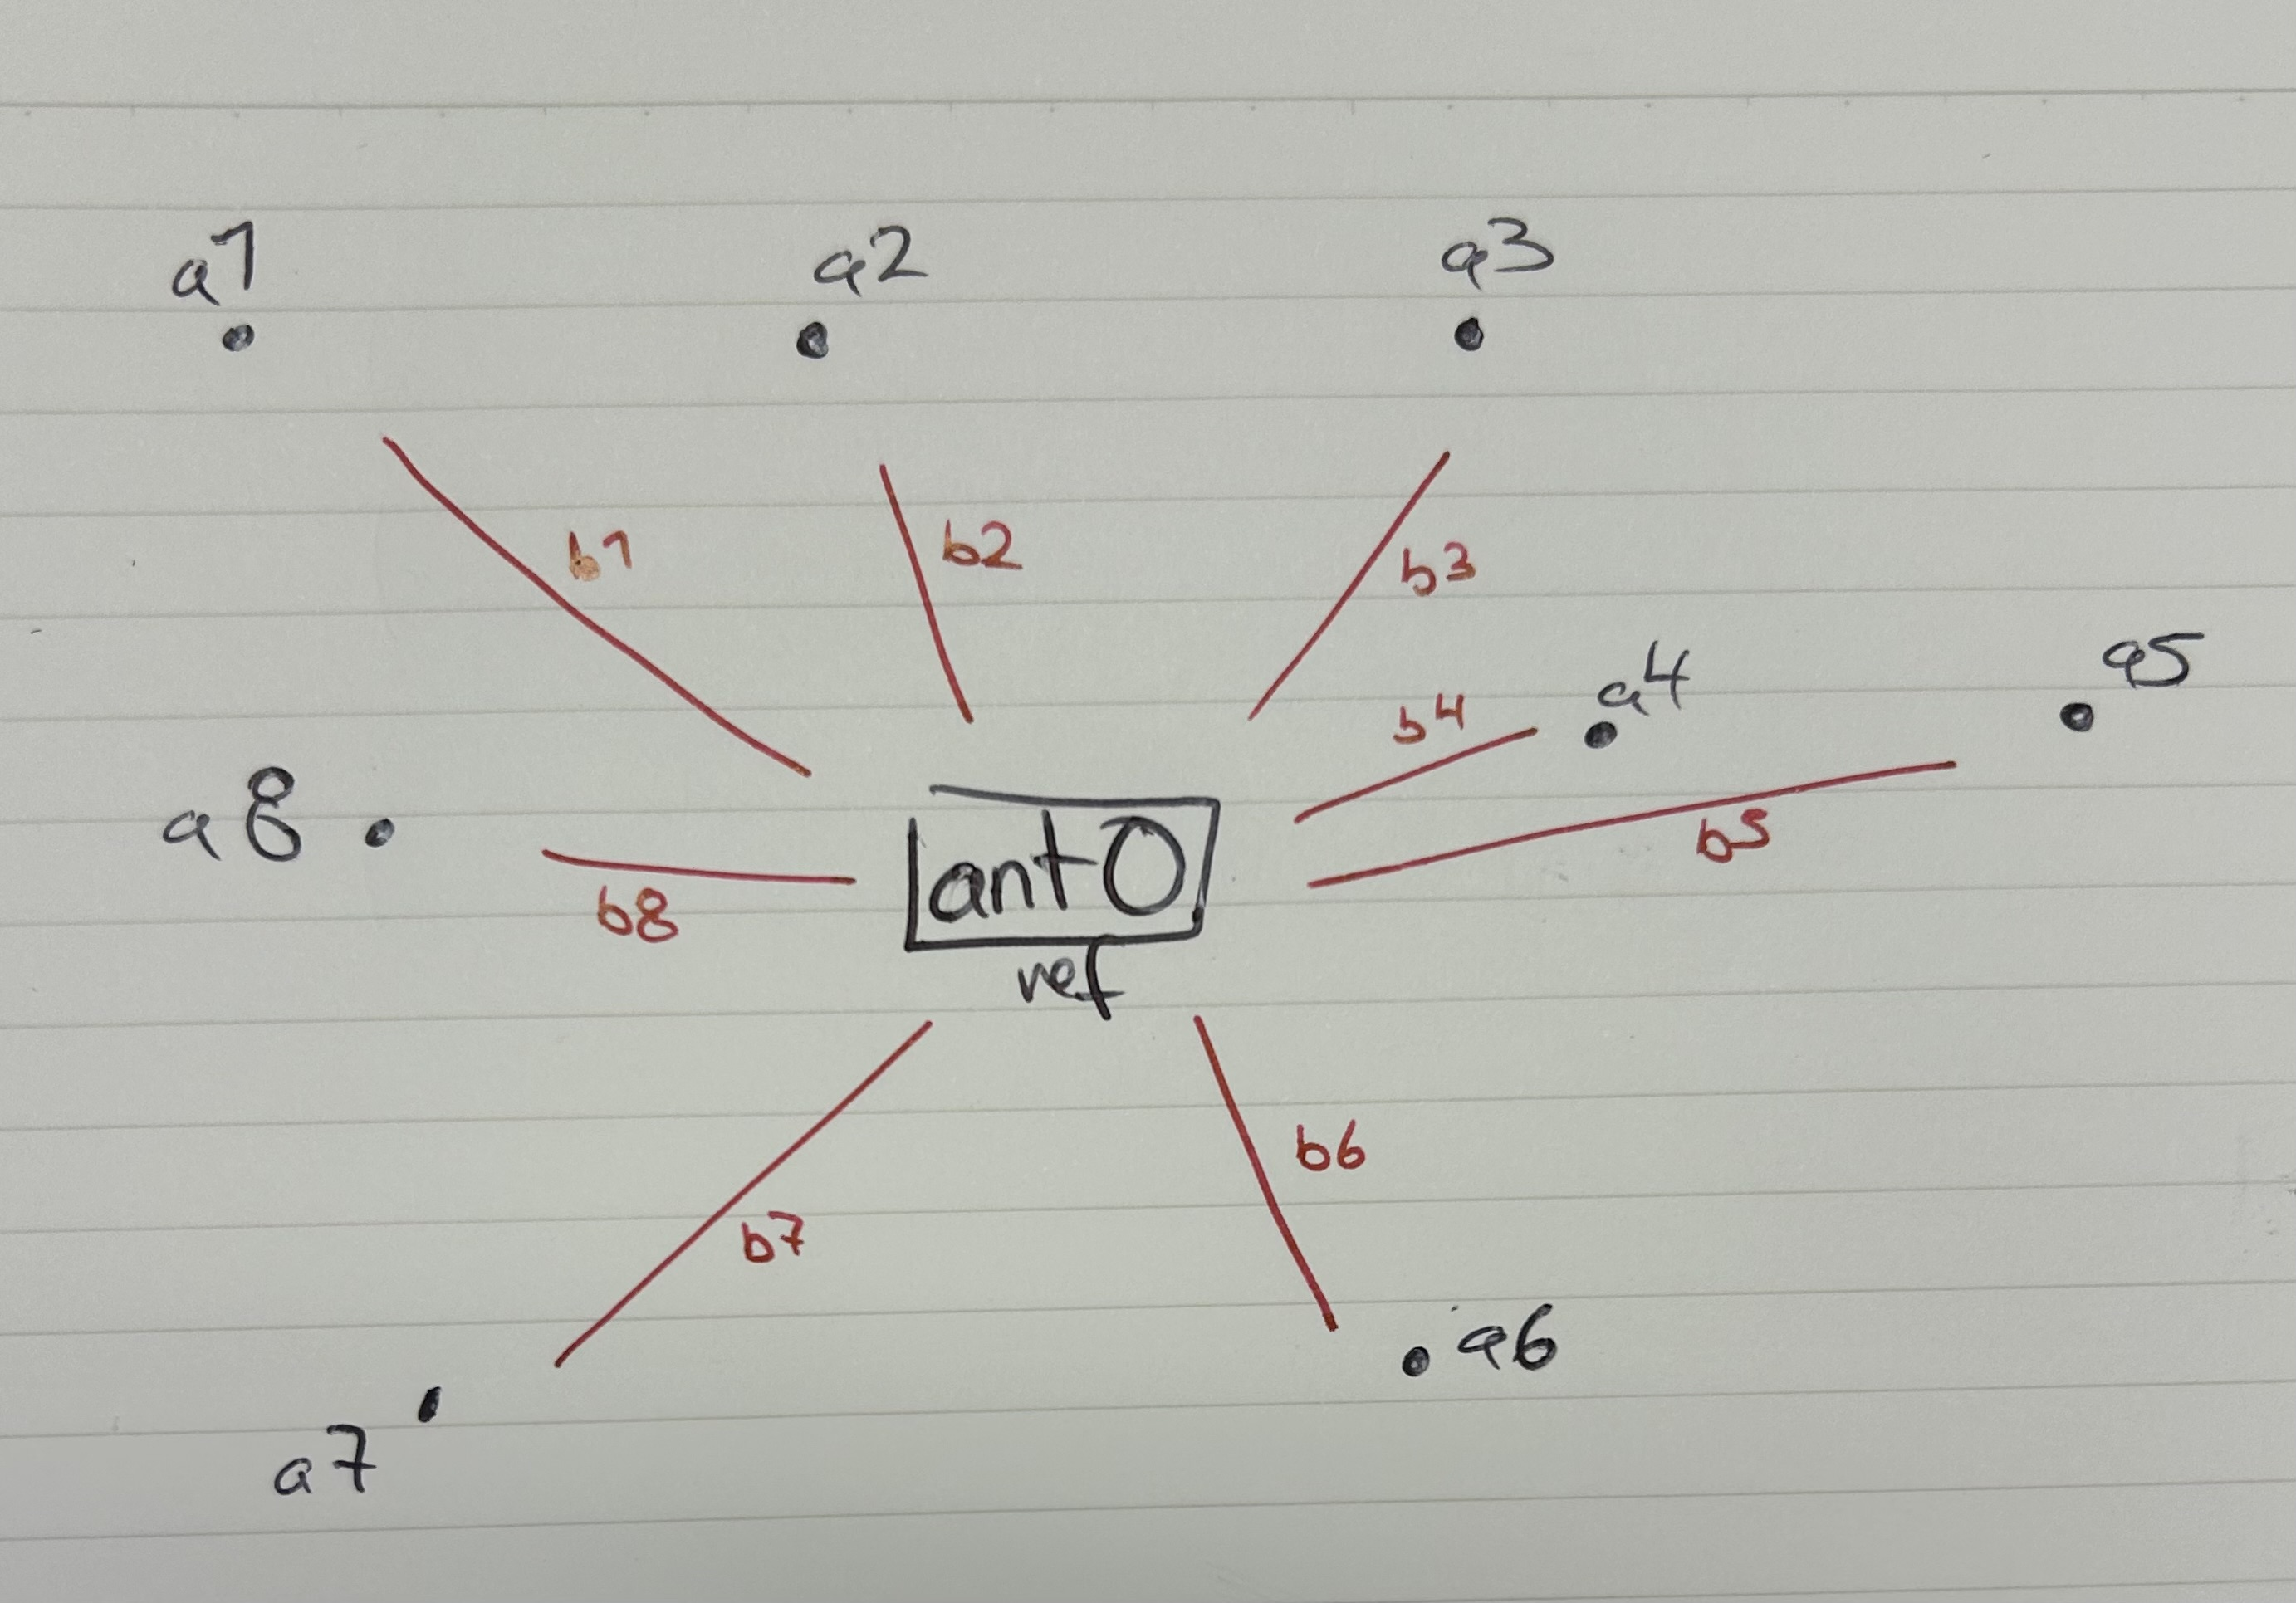
\includegraphics[width=0.5\linewidth]
  {Figures/baseline_array_placeholder.jpg}
  \caption{Example of Antenna Cluster. Reference Antenna need not be centrally positioned.}
  \label{fig:ant_cluster}
\end{figure}

We initially define a reference antenna (also referred to as Antenna 0), which will keep its initial estimated coordinates 
throughout the fitting. 
All other antenna are labeled with natural numbers 1, 2, 3, and so on. 
We only consider baselines originating from the reference antenna, and label them by the name of their connecting non-reference antenna. 
For example, as seen in Figure~\ref{fig:ant_cluster}, the baseline connecting Antenna 0 to Antenna 5 is labeled baseline 5.

Since we only require baseline vectors and not actual geodetic coordinates, a highly precise antenna position with respect to earth is 
of secondary importance. 
This allows us to fit each of these baselines individually and independently, using the non-reference coordinates as the only fitting parameter, 
determining the value which returns the best relative coordinates. 

With the general layout in mind, we observe the overall Baseline Calibration data flow in Figure~\ref{fig:flow}.

\begin{figure}[H]
    \centering
    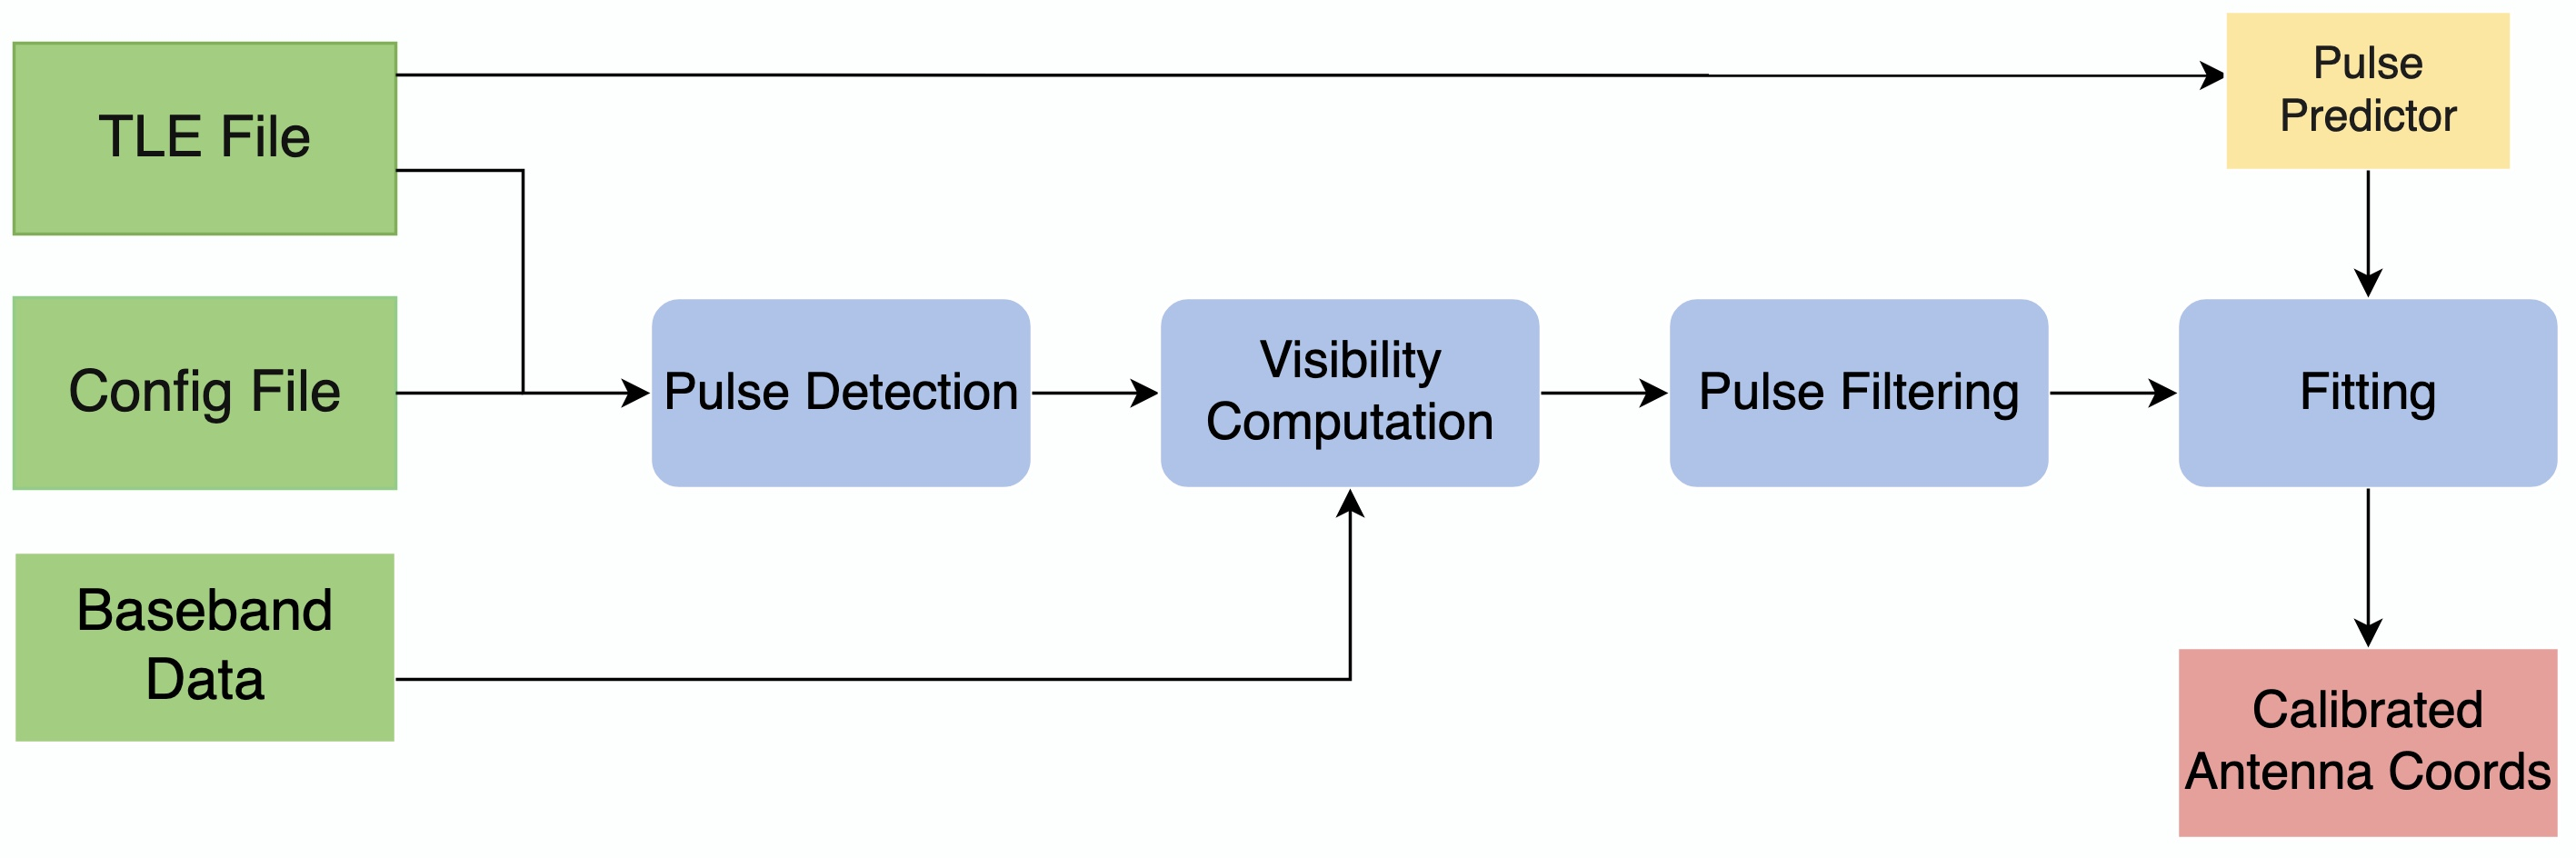
\includegraphics[width=\linewidth]{Figures/flowchart.jpeg}
    \caption{The Data flow is split into four main working modules (blue), 
    with three primary inputs (green), one fitting predictor function (yellow), and one primary output (red).}
    \label{fig:flow}
\end{figure}

Visibility Computation and filtering, the main observed data processing, are detailed in Section~\ref{sec:observed}. 
Phase prediction and synthesis is discussed in Section~\ref{sec:predicted}. 
Finally, the fitting process and its complications is outlined in Section~\ref{sec:fitting}. 
Since this process is still in development, we explain the future outlook in Section~\ref{sec:future}.

\section{Observed Pulses}
\label{sec:observed}

\subsection{Theoretical Pulse}

Let us again consider a single two-dimensional satellite pulse (shown previously in Figure~\ref{fig:sat_pulse}). 
We make assumptions of a flat sky, high satellite signal brightness, and uniform antenna response to simplify the theory.
Recall that we performed a cross cross correlation and found the exact spectrum number offset. 
Thus, using the raw baseband data, if we correct for known clock offset $\tau_c$ and perform direct cross correlation,
we will obtain complex visibilities with the geometric time delay $\tau_g$ encoded into them. This is derived below, using an integration time of $t_{\text{int}}$:
\begin{eqnarray}
    V_{0,1} &=& \int^{t_0 + t_{\text{int}}}_{t_0}  E_0(t) E_1^*(t) dt, \\\nonumber
    &=&  \int^{t_0 + t_{\text{int}}}_{t_0} E_0(t) \left[ E_0 (t) e^{2 \pi i \nu_0 \tau_g(t)} \right]^* dt,  \\\nonumber
    &=&  \int^{t_0 + t_{\text{int}}}_{t_0} E_0(t) E_0^*(t) e^{-2 \pi i \nu_0 \tau_g} dt, \\\nonumber
    &=&  e^{-2 \pi i \nu_0 \tau_g} \int^{t_0 + t_{\text{int}}}_{t_0} |E_0(t)|^2  dt
\end{eqnarray}
Here we assume that the satellite moves slowly with respect to the integration time, which allows us to extract the phase from the integral.
Therefore, we consider $\tau_g(t)$ to be constant for a single visibility computation. 
Thus, we have a complex visibility which has the geometric delay encoded into it, 
so for many pulses we can unwrap this phase and obtain a phase plot over time.
Moreover, even when not purely narrowband, we still expect a dominant presence of the $e^{-2 \pi i \nu_0 \tau_g}$ term as $E_0$ 
correlated with itself is very large.




\subsection{Practical Pulse}

Practically, we compute visibilities per chunk, blah blah

We use an accumulation length of $3*10^5$ spectra, with each spectrum having a period of approximately $16 \mu s$, 
leaving us with a chunk period of approximately $0.5s$. 
Usable sections of pulses usually last several minutes, meaning they typically contain between 500 and 1000 chunks.
i here is the index in the spectrum number, N is the accumulation length, i.e. length of chunk. 
\begin{eqnarray}
    V_{0,1,i} &=& \frac{1}{N} \sum_{i = 0} ^ {N-1} E_0[i]E_1[i] \\\nonumber
    &=& \frac{1}{N} \sum_{i = 0} ^ {N-1} \left| E_0[i] \right|^2 e^{2 \pi i \tau_g[i]}
\end{eqnarray}


Figure~\ref{fig:wrapped_phase} shows the angle with time for the visibility of all channels during a pulse. 
Can clearly see how the angle of the geometric time delay dominates channels index 2 and 3. 
 
\begin{figure}[H]
  \centering
  \begin{minipage}{0.45\textwidth}
    \centering
    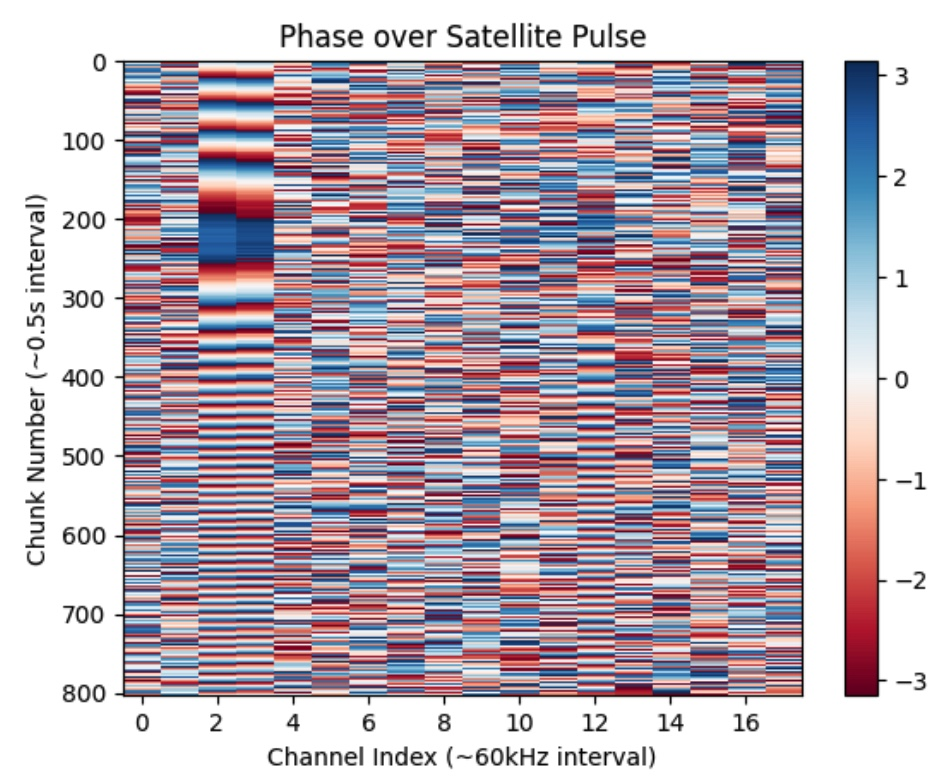
\includegraphics[width=\linewidth]{Figures/wrapped_phase_example.jpeg}
    \caption{Wrapped visibility phase. The satellite pulse is visible in channels 2 and 3.}
    \label{fig:wrapped_phase}
  \end{minipage}
  \hfill
  \begin{minipage}{0.45\textwidth}
    \centering
    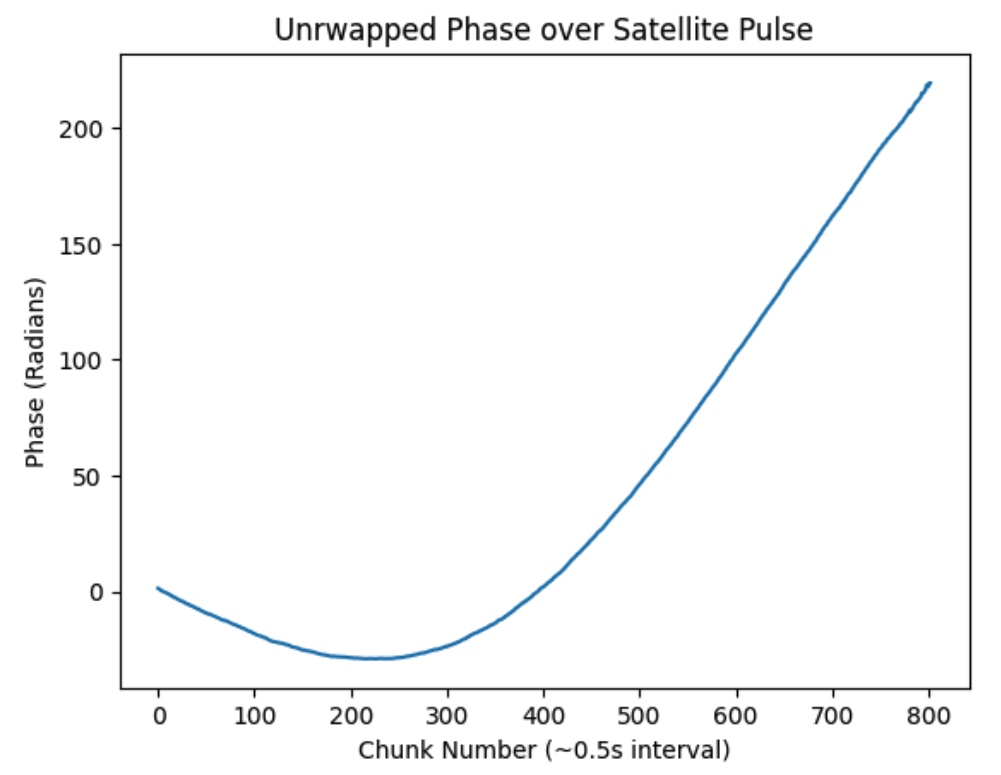
\includegraphics[width=\linewidth]{Figures/unwrapped_phase_example.jpeg}
    \caption{Unwrapped phase for channel 2 over the entire pulse.}
    \label{fig:unwrapped_phase}
  \end{minipage}
\end{figure}


To obtain the observed phase for each satellite pulse, we must use the satellite detection script 
(outlined in Chapter~\ref{chap: timing}) to get the pulse times, channels, and the spectrum number offsets. 
Spectrum number, of course, being our proxy for time. 
We correct for this as our clock offset $\tau_c$. 
Once this information is recorded and implemented, we can correlate Baseband data from the reference 
and non-reference antenna to obtain raw visibilities. We do this for each pulse, for each day of data, and for each baseline.


The unwrapped phase is the final product of the visibility computation, and will be used as our observed data 
for the eventual coordinate fit. 
For each baseline, the total observed data is compromised of several such unwrapped pulse phase curves. 


\subsection{Filtering}

Oftentimes, the visibility will be rather messy.
The pulse filtering process ensures we obtain a continuous, reasonably smooth phase plot.
It involves the following steps:

\begin{enumerate}
  \item There is often missing data in the 1bit visibilities, due to a lack of data in the chunk. We interpolate over the complex data
        directly to ensure the visibility is continuous.
  \item When unwrapping the phase, there are some parts of the pulse that have almost no distinguishable phase, and must be cut out.
  \item Finally, in the good portions of the phase, there can be jagged jumps, which are interpolated over smoothly (in visibility?). 
        this is either caused by bad data or by aliasing (since the satellite phase angle can change very fast).
\end{enumerate}

For the time being, this is all conducted manually. 
The aim is to automate this process to improve reproducability and speed.



\section{Predicted Phase}
\label{sec:predicted}

In order to correctly fit the non-reference antenna's coordinates, we must construct a function which 
accurately predicts the satellite pulse phase over time. 
Its only free parameter must be the non-reference antenna's coordinates. 
Once we have constructed this function, we can evaluate the \textit{goodness of fit} of the initial guess coordinates as a preliminary test. 
This can be seen in Figure~\ref{fig:unfitted}.


\begin{figure}[H]
  \centering
  \begin{minipage}{0.45\textwidth}
    \centering
    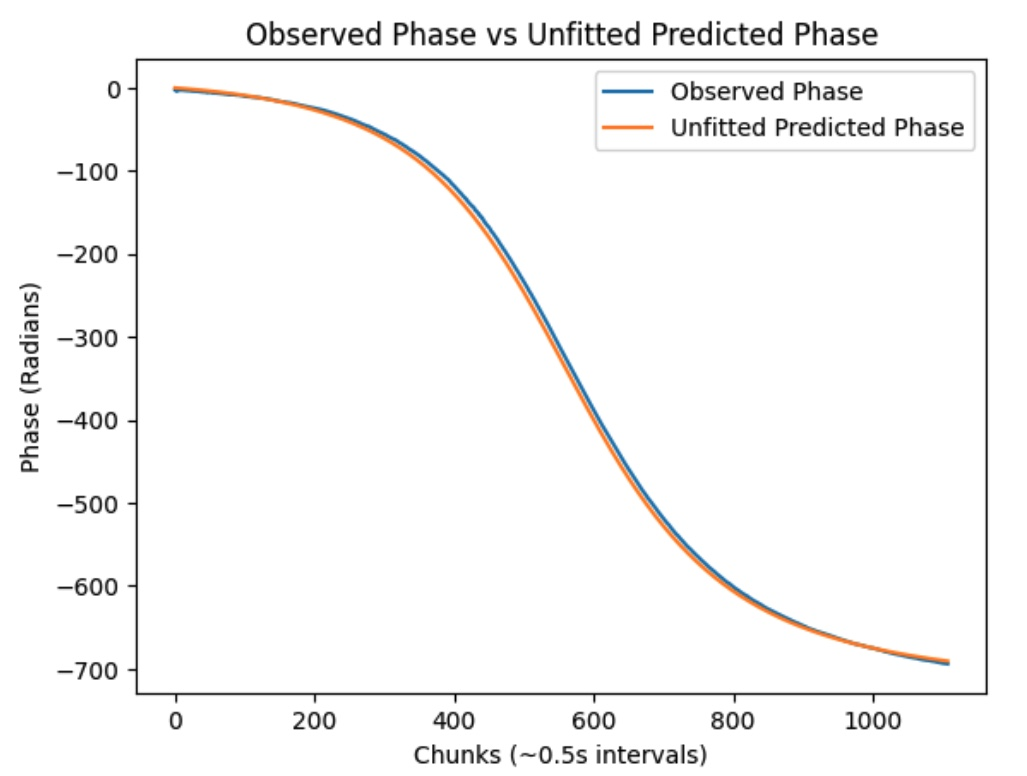
\includegraphics[width=\linewidth]{Figures/observed_vs_unfitted_predicted_phase.jpeg}
  \end{minipage}
  \hfill
  \begin{minipage}{0.45\textwidth}
    \centering
    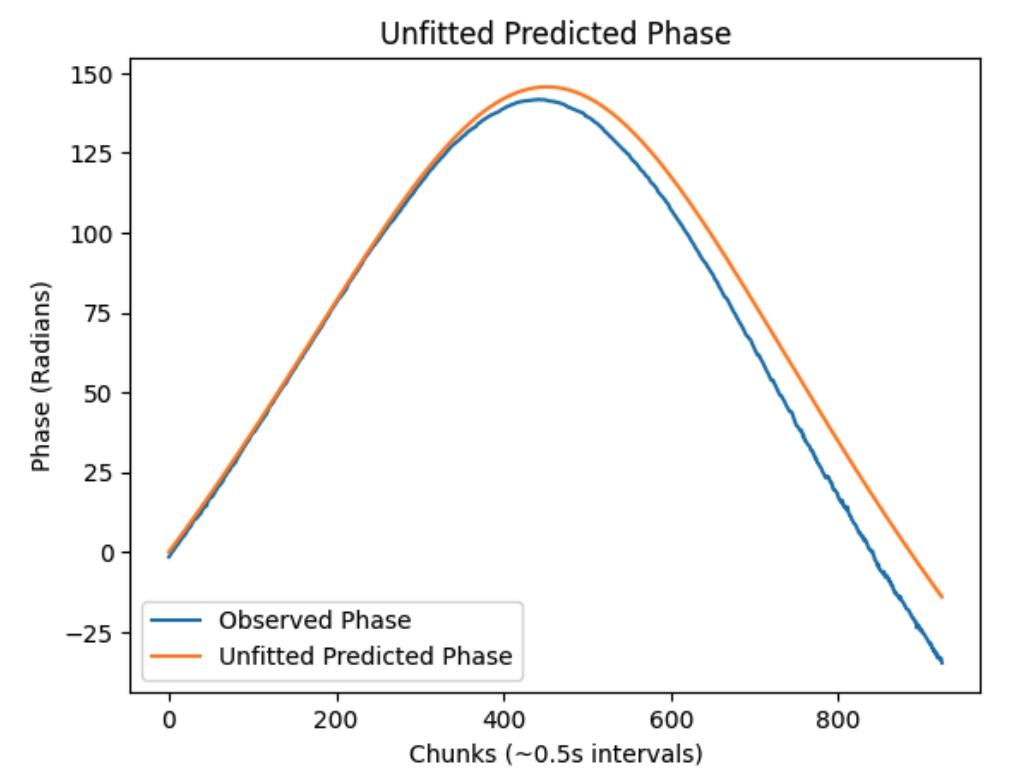
\includegraphics[width=\linewidth]{Figures/obs_vs_unfitted_pred_2.jpeg}
  \end{minipage}
  \caption{Two examples of unfitted predicted phases against their observed counterparts.}
  \label{fig:unfitted}
\end{figure}

Figure~\ref{fig:unfitted} illustrates the necessity of fitting for multiple satellite passes simultaneously, 
as different satellites will have different trajectories in the sky, and thus will favor different fits.





\section{Fitting}
\label{sec:fitting}

%notes to add

% - question of directionality
% - 

\subsection{Moving Parts}

There are several things we need to take into account during the fitting process. 

First of all, we must take into account the thermal noise on each pulse. The residuals of each pulse must be weighted using the noise of the pulse, to ensure that noisy pulses are considered less.

Secondly, we must ensure that our various pulses cover several different directions in the sky. A baseline is a single line, so passes have to move over at different angles to properly calibrate it. DEVELOP?


\begin{figure}[H]
    \centering
    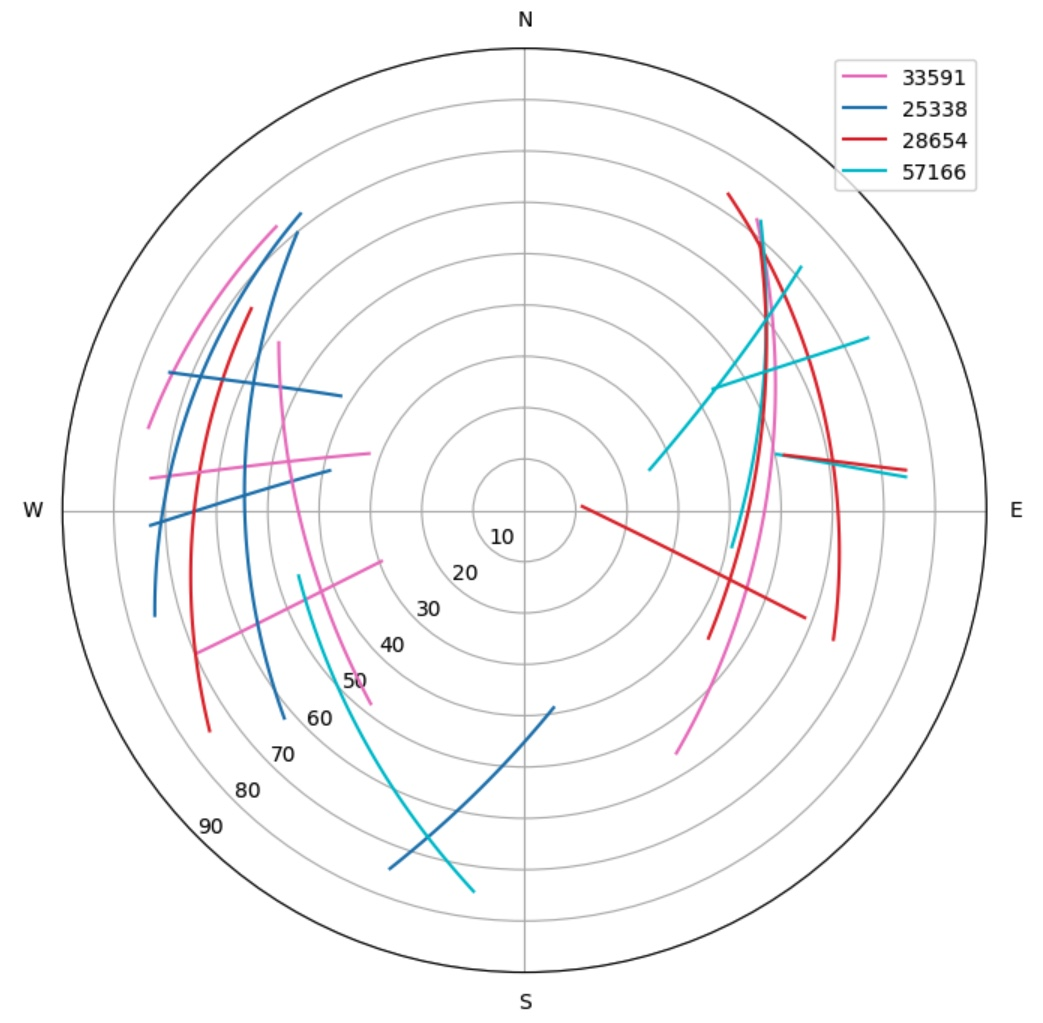
\includegraphics[width=0.4\linewidth]{Figures/satpass_plot.jpeg}
    \caption{Example of a satellite pulse plot, in direction over the sky}
    \label{fig:satpulse_plot}
\end{figure}


Finally, we must take into account offset between predicted phases and observed phases. We assume that when we predict a phase, it is accurate in human observer time. We also assume (and pray) that the visibility spectrum number offset correctly aligns the two clocks of the two antenna. This is done in such a way that leaves Antenna 0's clock unchanged, and shifts the spectra of Antenna 1 (which makes sense or else it would be super confusing with multiple antenna). But we know that there is significant clock drift in the human time (RPI) clock of the Antenna. Since each pulse is accessed separately using human time, each pulse has the risk of having a time offset associated to it. So we must implement a per-pulse time offset variable that can correct for this. 

Therefore, the fitting process has three separate weighting methods, alongside three separate fitting types. These are modular; any fitting method can be used with any of the weighting methods. 



\subsection{Weighting Methods}


\subsection{Fitting Methods}

We do several types of fits. First is only with coordinates.

Obtain residuals from each pulse, concatenate into one large array, and least squares fit with your predictor function. Only fitting parameter is the coordinate for the predicted phase. This is done simultaneously for all considered pulses.

This gives us one possible fit for one baseline. 


%lowkey here you don't have to spam a bunch of plots
Figure~\ref{fig:obs_vs_fitted_all} shows six pulses with their fitted phases. 

\begin{figure}[H]
    \centering
    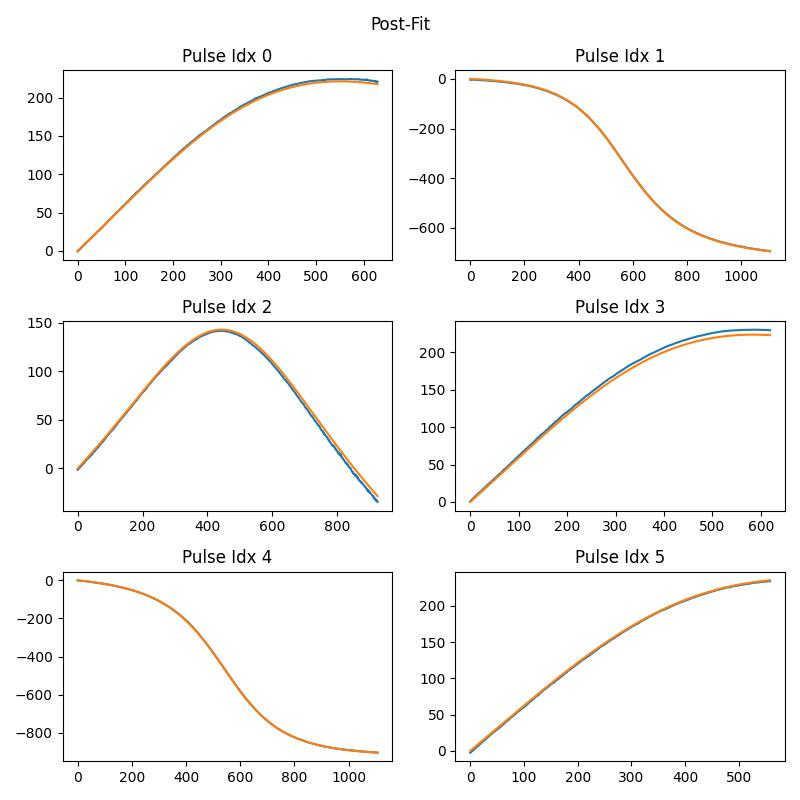
\includegraphics[width=0.7\linewidth]{Figures/post_fit_calib_plots_tlm_1721900002.jpg}
    \caption{Fitted with the TRF method. In this run, TRF and LM gave negligibly different results.}
    \label{fig:obs_vs_fitted_all}
\end{figure}

We can see how Pulse Index 1 (seen unfitted in Figure~\ref{fig:obs_vs_unfitted}) has very close agreement between observed and predicted phases. This is further exemplified in the residuals plots, seen in Figure~\ref{fig:resids_all}.

\begin{figure}[H]
    \centering
    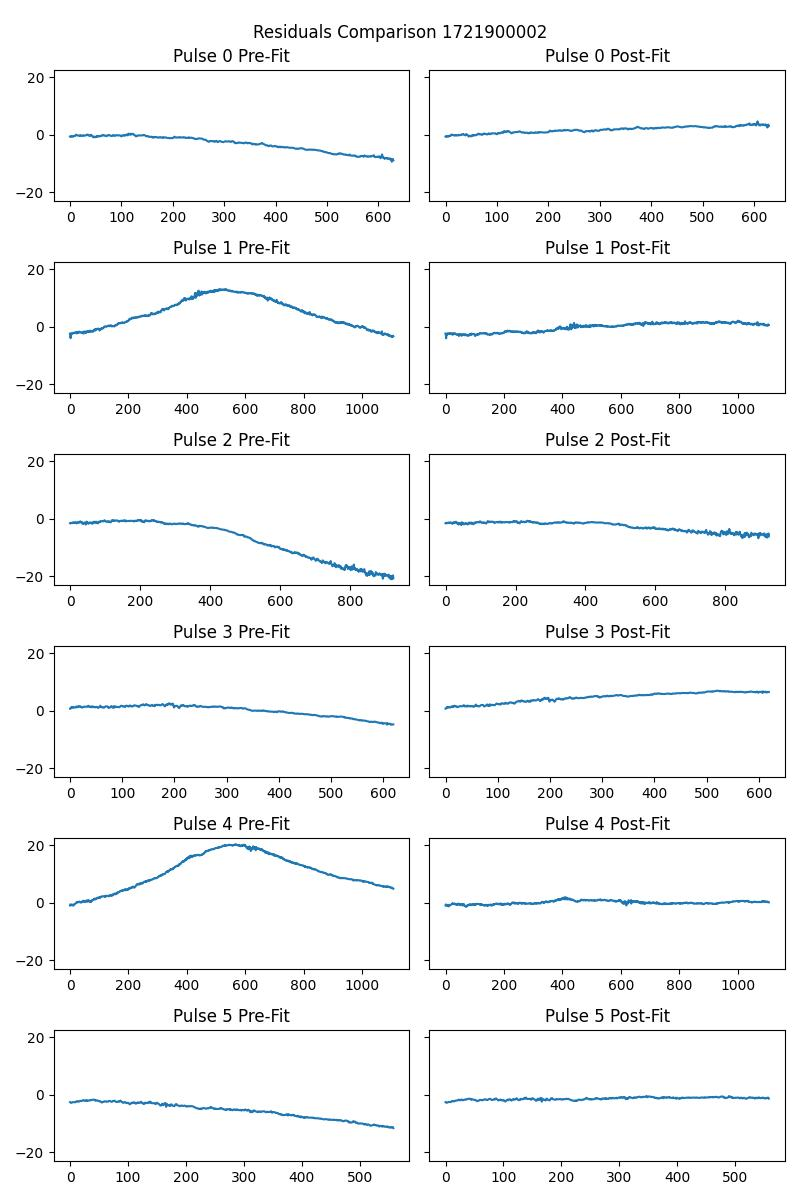
\includegraphics[width=0.5\linewidth]{Figures/residuals_individual_tlm_coordfit_1721900002.jpg}
    \caption{All pulses with residuals before and after fitting. Again with TRF algorithm.}
    \label{fig:resids_all}
\end{figure}


Secondly, we have a per-pulse time offset fit. The reason for this is the time discrepancy (in human observer time) between getting 


\subsection{Testing Methods}

To ensure we have found a valid coordinate, we must conduct some testing. Naturally, this means varying some fixed parameters and ensuring our coordinates converge to the same values. 

First, we must vary the initial guess for the non-reference antenna. This ensures that the fit is not stuck in a local minimum. In testing, several randomly generated nearby coordinates are also tested, and their results are compared. For a coordinate to be deemed valid, they must all return negligible differences in coordinates.

Second, we utilize two fitting methods as a safety check. We use both the 'Trust Region Reflective' and 'Levenberg-Marquardt' algorithms of least squared fitting. For a coordinate to be deemed valid, both fit method must yield a negligible differences. 

Third, we fit over multiple sets of 5-6 pulses, and vary combination of satellites. This ensures there is no bias in pulse direction, satellite type, or time of day. A valid coordinate must, as for other variables, remain consistent across pulses.

These tests are conducted for each baseline, using the single baseline coordinate calibration script.




\section{Limitations and Future Development}
\label{sec:future}

As of the writing of this section, there are several technical limitations causing difficulties in the development of a streamlined, generalized coordinate calibration script.

The main issue is the inconsistency in observed phase plots. This is the result of low SNR satellite passes (which are detected but not good), unwrapping bugs, or missing data. This means pulses must be combed through manually before being passed through the calibration script, significantly slowing analysis. Figures~\ref{fig:bad_pulse_phase1} and ~\ref{bad_pulse_phase2} provide an example of such a pulse.

This issue will be resolved before making a generalized script that can fit and test coordinates multiple baselines automatically. This would be the optimal case, and would significantly facilitate any future project's baseline optimization.



\chapter{Visibilities and Storage}
\label{chap:visibilities_and_storage}

Now that we have timing and positioning figured out, it's time to compute visibility data.
We re-pfb our channelized data before applying a cross-correlation, explained in XXXX.
We save data as a pyuv format, which is detailed in XXXX.

\section{Re-PFB}

Main idea is to take our baseband data. It is already channelized, but coarsely. 
We Inverse PFB it, and return to (approximately) the voltage-time data.
We then apply another PFB, with some oversampling constant.
Get finer channels, and also specify a certain region we want to look at.
We then cross-correlate and get our visibilities with the oversampled channel resolution.
This is a better method because....

In our case, we use these numbers XXXX


\section{PYUV}

%intro sentence
The cross correlation gives us plenty of data.
%motivation
We save everything in the specific PYUV format which allows for saving several baselines and spectral windows,
while having relatively simple handling and updating.

Below is an outline of the main objects in such files, and the conventions we use for them.


\subsection{Constants}


\begin{table}[H]
\centering
\begin{tabular}{|l|p{15cm}|}
\hline
\textbf{Field} & \textbf{Description} \\
\hline
\texttt{Nbls} & Number of baselines. \\
\hline
\texttt{Ntimes} & Number of times. \\
\hline
\texttt{Nblts} & Number of baseline-times. Not necessarily equal to \texttt{Nbls} $\times$ \texttt{Ntimes}. \\
\hline
\texttt{Nfreqs} & Number of frequency channels. \\
\hline
\texttt{Npols} & Number of polarizations. \\
\hline
\texttt{Nspws} & Number of spectral windows. \\
\hline
\texttt{Nphase} & Number of phase centers in the data. \\
\hline
\texttt{Nants\_data} & Number of antennas with data present (i.e., number of unique entries in \texttt{ant\_1\_array} and \texttt{ant\_2\_array}). May be smaller than the number of antennas in the array. \\
\hline
\texttt{vis\_units} & Visibility units. Options are: \texttt{"uncalib"}, \texttt{"Jy"}, or \texttt{"K str"}. \\
\hline
\end{tabular}
\caption{Key PYUV parameters. Will determine much of the rest.}
\end{table}


\subsection{Data}

\subsubsection{Visibility-Related}

Explain how baseline-times are arranged??? How to extract data??

\begin{table}[H]
\centering
\begin{tabular}{|l|l|l|p{5cm}|}
\hline
\textbf{Name} & \textbf{Shape} & \textbf{Type} & \textbf{Description} \\
\hline
\texttt{data\_array} & (Nblts, Nfreqs, Npols) & complex float & Visibility data in units of \texttt{vis\_units} \\
\hline
\texttt{flag\_array} & (Nblts, Nfreqs, Npols) & bool & True indicates flagged data \\
\hline
\texttt{nsample\_array} & (Nblts, Nfreqs, Npols) & float & Number of samples included in the visibility chunk\footnotemark[1] \\
\hline
\end{tabular}
\caption{Where the visibility information lives.}
\end{table}

\footnotetext[1]{Also often used to check for flagging.}

\subsubsection{Time-Related}
\begin{table}[H]
\centering
\begin{tabular}{|l|l|l|l|}
\hline
\textbf{Name} & \textbf{Shape} & \textbf{Units} & \textbf{Description} \\
\hline
\texttt{time\_array} & (Nblts) & Julian Date & Time at center of integration. \\
\hline
\texttt{lst\_array} & (Nblts) & radians & Local Apparent Sidereal Time (LAST). \\
\hline
\texttt{integration\_time} & (Nblts) & seconds & Duration of each visibility integration. \\
\hline
\end{tabular}
\caption{Time-related data. Required to reconstruct time information from \texttt{data\_array}}
\end{table}

\subsubsection{Baseline-Related}
\begin{table}[H]
\centering
\begin{tabular}{|l|l|l|l|}
\hline
\textbf{Name} & \textbf{Shape} & \textbf{Type} & \textbf{Description} \\
\hline
\texttt{ant\_1\_array} & (Nblts) & int & First antenna in baseline. \\
\hline
\texttt{ant\_2\_array} & (Nblts) & int & Second antenna in baseline. \\
\hline
\texttt{baseline\_array} & (Nblts) & int & Encodes ant1 and ant2 (we use: $2048 \times \texttt{ant1} + \texttt{ant2} + 2^{16}$)\footnotemark[2]. \\
\hline
\end{tabular}
\caption{Antenna and baseline data. Also required to reconstruct baseline information from \texttt{data\_array}}
\end{table}

\footnotetext[2]{This special code is for compatibility with other data formats, and for efficiency in sorting methods.}

\subsubsection{Frequency and Polarization}
\begin{table}[H]
\centering
\begin{tabular}{|l|l|l|l|}
\hline
\textbf{Name} & \textbf{Shape} & \textbf{Units/Type} & \textbf{Description} \\
\hline
\texttt{freq\_array} & (Nfreqs) & Hz & Center frequency of each channel. \\
\texttt{channel\_width} & (Nfreqs) & Hz & Width of each frequency channel. \\
\texttt{polarization\_array} & (Npols) & int & Polarization codes.\footnotemark[3] \\
\hline
\end{tabular}
\caption{Spectral and polarization data.}
\end{table}

\footnotetext[3]{Different integers serve to represent which exact polarization we are working with. 
Will not go through it here, see AIPS Memo 117}


\subsubsection{Spectral Window}
\begin{table}[H]
\centering
\begin{tabular}{|l|l|l|l|}
\hline
\textbf{Name} & \textbf{Shape} & \textbf{Type} & \textbf{Description} \\
\hline
\texttt{spw\_array} & (Nspws) & int & Spectral window identifiers. \\
\texttt{flex\_spw\_id\_array} & (Nfreqs) & int & Maps frequencies to spectral windows. \\
\hline
\end{tabular}
\caption{Spectral window information.}
\end{table}



\section{Storage System}

How the pyuv files work (includingconventions for storage), 
what the storage system is, and how to access them (with examples!).


\chapter{Fine Timing}
\label{chap:fine_timing}




\end{document}